\documentclass[12pt,letterpaper]{article}

%% -packages-
\usepackage{graphics}
\usepackage{psfrag}
\usepackage[round]{natbib}
\usepackage{longtable}
\usepackage{rotating}
\usepackage{rotate}
\usepackage{lscape}
\usepackage{amssymb}
\usepackage{amsmath}
\usepackage[colorlinks,citecolor=black,bookmarks]{hyperref}
\usepackage{color}
\usepackage{multicol}
\usepackage{alltt}
\usepackage{setspace}
\usepackage{lineno}


%\usepackage[latin1]{inputenc} % To use characters such as � without typing \'e
%\usepackage[cyr]{aeguill} % To display characters such as �
%\usepackage{xspace} % To get the right spacings in front of : and so on
\usepackage[french,english]{babel}

%% ---------------------------------------------------------------------
%%Page Layout Properties-------------------------------------------------

%\voffset 0in \textwidth 7.0in  \oddsidemargin 0in
%\evensidemargin 0in \headheight 0.in \textheight 9in  %%Look at Box13.1 for text scale
\voffset -0.75in
\hoffset -0.75in
\textwidth 6.5in%
\textheight 9.0in%
%\evensidemargin 0.in%

%\textwidth 6in%
%\topmargin 0in%
\setlength{\LTcapwidth}{\textwidth} %caption width for longtables

%Arial font
\renewcommand{\rmdefault}{phv} % Arial
\renewcommand{\sfdefault}{phv} % Arial

%Logo
%\usepackage{fancyhdr}
%\renewcommand{\headheight}{0.6in}
%\setlength{\headwidth}{\textwidth}
%\fancyhead[L]{}% empty left
%\fancyhead[R]{ % right
%   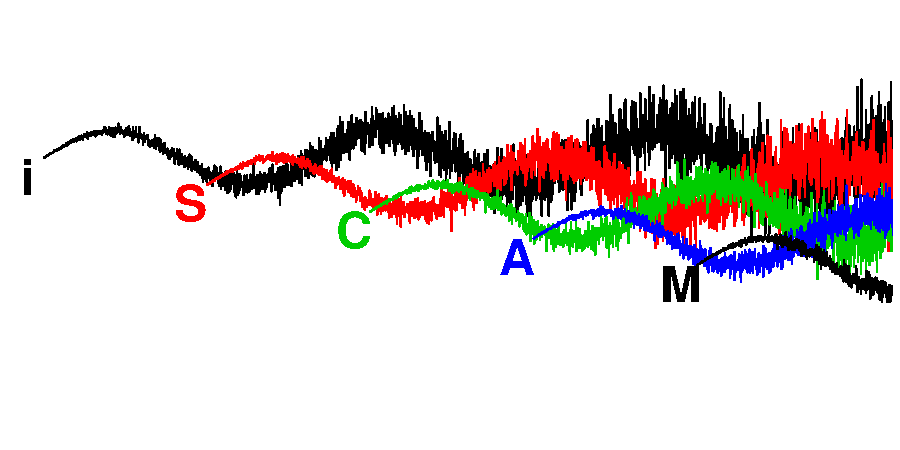
\includegraphics[height=0.53in]{iscamlogo.eps}
%}
%\pagestyle{fancy}


%-------------------------------------------------------------------------
%Water mark
%%\usepackage{eso-pic}
%%\usepackage{graphicx}
%%\usepackage{color}
%%\usepackage{type1cm}
%%\usepackage{float} 
%%
%%\makeatletter
%%  \AddToShipoutPicture{%
%%    \setlength{\@tempdimb}{.5\paperwidth}%
%%    \setlength{\@tempdimc}{.5\paperheight}%
%%    \setlength{\unitlength}{1pt}%
%%    \put(\strip@pt\@tempdimb,\strip@pt\@tempdimc){%
%%      \makebox(0,0){\rotatebox{45}{\textcolor[gray]{0.85}{\fontsize{1.75cm}{1.75cm}\selectfont{DRAFT  \today}}}}
%%    }
%%} \makeatother


%% -math-
\newcounter{saveEq}
  \def\putEq{\setcounter{saveEq}{\value{equation}}}
  \def\getEq{\setcounter{equation}{\value{saveEq}}}
  \def\tableEq{ % equations in tables
    \putEq \setcounter{equation}{0}
    \renewcommand{\theequation}{T\arabic{table}.\arabic{equation}}
    \vspace{-5mm}
    }
  \def\normalEq{ % renew normal equations
    \getEq
    \renewcommand{\theequation}{\arabic{section}.\arabic{equation}}}

  \def\puthrule{ %thick rule lines for equation tables
    \hrule \hrule \hrule \hrule \hrule}


%%\newcommand{\msy}{$C^*$}
%%\newcommand{\fmsy}{$F^*$}
%%\newcommand{\sbmsy}{$\rm{SB_{MSY}}$}
%%\newcommand{\sbfour}{$\rm{SB_{40}}$}
%%\newcommand{\�}{\'e}
%%\newcommand{\�}{\`e}
%%\newcommand{\�}{\`a}
%%\newcommand{\�}{\^e}
\newcommand{\iscam}{
{$^i$}\textcolor{red}{S}\textcolor{green}{\small{}C}{\textcolor{blue}{\footnotesize{}A}}\textcolor{black}{$_\textnormal{M}$}}%{\raisebox{-0.7ex}{M}}%

\newcommand{\fmsy}{F$_{\textnormal{MSY}}$}
\newcommand{\bmsy}{B$_{\textnormal{MSY}}$}

%% ---------------------------------------------------------------------

\title{
Use of natural cubic spline interpolation for estimating selectivity parameters in statistical catch-age models.
\vfill}

\author{Steven J. D. Martell$^1$\\ and\\ James N. Ianelli$^2$\\
\\
$^1$University of British Columbia, Fisheries Centre,\\ 
2202 Main Mall, Vancouver, BC V6T 1Z4, Canada. \\
\texttt{s.martell@fisheries.ubc.ca}\\
\\
$^2$National Marine Fisheries Service, NOAA, \\
7600 Sand Point Way NE Seattle WA 98115, USA\\
\texttt{Jim.Ianelli@noaa.gov}\\
}


\begin{document}
\doublespace

    \maketitle \thispagestyle{empty} \clearpage

%%
 \selectlanguage{english}

    %\input{ToDoList}
%% -Executive summary material------------------------------------------
\linenumbers
\begin{abstract}
The estimation of selectivity, or the fraction of an age or size class of fish that are vulnerable to fisheries exploitation, is critical in statistical catch age models.  Selectivity defines what ages or sizes of fish are removed from the population and also defines, for example, MSY-based reference points. Assumptions about selectivity have ranged from simple, two parameter time-invariant asymptotic functions, to random walks,  to an extremely complex array of time-varying age-specific selectivity coefficients for nearly every age-class in each year.  There is little doubt that selectivity can change over time with refinements in fishing gears, range expansions/collapse of areas fished and even the impacts of regulation on fishing behaviour.  We present an alternative method that attempts to estimate a reduced number of distinct knots and interpolate age-specific selectivities using cubic splines and bicubic splines.  We apply the method to simulated data to demonstrate that it is in fact possible to estimate time-varying changes in age-specific selectivity. We also apply the method to the Pacific hake data from the Northeast Pacific.
\end{abstract}
\clearpage

%% -Main body of the document-------------------------------------------
\section*{Introduction}
Most of the major fish stock assessments are based on the analysis of age or size composition data, where the hope is that the age-composition data provide information on: age selectivity, cumulative mortality, and recruitment or relative cohort strengths \citep{WalMart2004}.  There are two general approaches to the analysis of catch-age data, virtual methods that propagate numbers-at-age backwards in time (e.g., Virtual Population Analysis, or VPA) and Statistical Catch Age (SCA) methods that propagate numbers-at-age forward in time \citep{gavaris2002sif}.  VPA methods tend to make fewer assumptions about selectivity in comparison to SCA methods; estimates of selectivity are only required for the incomplete cohorts (i.e., the age-classes that still persist in the fishery).  Statistical Catch Age models, however, rely heavily on the concept of separability where fishing mortality has an age-effect and a year effect.  Simpler assessments usually assume that the age-effect (or selectivity) is constant over time, implying that the fishery operations (e.g., locations fished and gear fished) also remains constant over time.  In many cases we know that fishing operations have changed over time and these operational changes can have large effects on selectivity.  Without full knowledge of operational changes, assumptions of constant selectivity can lead to overly optimistic forecasts of abundance.

The collapse of the 2J3KL Atlantic cod (\textit{Gadus moruha}) is a classic example of changes in selectivity associated with changes in the spatial distribution of trawl effort.  In the late 1980s and 1990, when the trawl fleet was unable to catch fish in the traditional trawling grounds, the fleet moved inshore and target smaller immature cod.  This was initially interpreted as a large recruitment event owing to the large number of age-3 fish showing up in the catch age-data.  Another example of changes in selectivity relating to changes in fisheries management plans was the establishment of species specific Total Allowable Catches (TAC) off the west coast of British Columbia in 1997; if any one species TAC was achieved then the entire fishery would be shut down for the season.  In this case, the BC trawl fishery began to actively avoid catching species with limited TACs.  For example, Pacific cod (\textit{Gadus macrocephalus}) were normally captured during the spawning season, but due to small TACs for this species, the fishery avoided the traditionally fished spawning grounds and captured fewer and smaller cod.  The size composition data for landed Pacific cod rapidly shifted to a much smaller size distribution that could easily be interpreted as a large recruitment under the assumption of constant selectivity.

In recognition of changes in age effects associated with changes in fishing operations and or availability of specific year classes, statistical models with explicit time-varying changes in selectivity have been developed \citep[e.g.,][]{butterworth2003statistical}, and have been shown in simulation studies to perform just as well when the true selectivity is actually constant over time \citep{radomski2005comparison}. \cite{radomski2005comparison} also demonstrated time varying changes in selectivity performed much better than constant selectivity models when in fact the true selectivity does change over time, even at the expense of additional estimated model parameters.  

Another substantial problem with SCA models and selectivity is the confounding between dome-shaped selectivity and natural mortality \citep[e.g.,][]{thompson1994confounding}.  The disappearance of older age-classes in age-composition data can usually be explained equally well with low natural mortality rates and increased fishing mortality associated with an asymptotic increase in selectivity-at-age, or high natural mortality rates and decreased fishing mortality associated with declines in selectivity at older ages (i.e., dome-shaped selectivity).  

\citep{aanes2007estimation}


\bibliographystyle{apalike}
\bibliography{$HOME/Documents/ARTICLES/Articles-1}

%% -Appendix material Model Description --------------------------------
%\newpage
%\appendix
%	\section{Statistical functions \& probability distributions}
\begin{multicols}{2}
Many of the statistical functions commonly used in R have been written as negative log likelihoods and are in the \texttt{stats.cxx} library.  In this appendix is the documentation for the available functions in the stats.cxx library.  For the most part I have implemented the function based on the description from the R language, so it is possible to use \texttt{?function} name in R to learn more about the funciton.  Here I provide the formula, the actual code used to implement the function and a description of the variables. Note that some of the functions have been overloaded several times to deal with variables, vectors or a matrix.
\end{multicols}

\paragraph{dbeta} The beta distribution.
\[
	p(x|a,b) = - \ln(\Gamma(a+b))+(\ln(\Gamma(a))+\ln(\Gamma(b)))-(a-1)\ln(x)-(b-1)*\ln(1-x)
\]
the mean is given by $a/(a+b)$ and the variance is $\dfrac{ab}{(a+b)^2(a+b+a)}$
\begin{verbatim}
//beta distribution
dvariable dbeta(const dvariable& x, const double a, const double b)
{
	return - gammln(a+b)+(gammln(a)+gammln(b))-(a-1.)*log(x)-(b-1.)*log(1.-x);
}
\end{verbatim}

\paragraph{dgamma} The gamma distribution.
\[
 p(x|a,b) = -a \ln(b)+\ln(\Gamma(a))-(a-1)\ln(x)+bx
\]
where the mean and variance are given by $E(x) = ab$ and $Var(x) = ab^2$. The following code is implemented in \texttt{stats.cxx} library:
\begin{verbatim}
//gamma
dvariable dgamma(const dvariable &x, const double a, const double b)
{
	return -a*log(b)+gammln(a)-(a-1.)*log(x)+b*x;
}
\end{verbatim}


\paragraph{dnorm} The normal distribution
\[
	p(x|\mu,\sigma) = 0.5\ln(2\pi)+\ln(\sigma)+0.5\frac{(x-\mu)^2}{\sigma^2}
\]
where the mean is $\mu$ and the variance is $\sigma^2$.
\begin{verbatim}
//normal distribution
dvariable dnorm(const dvariable& x, const double& mu, const double& std)
{
	double pi=3.141593;
	return 0.5*log(2.*pi)+log(std)+0.5*square(x-mu)/(std*std);
}
\end{verbatim}

\paragraph{dlnorm} The log normal distribution
\[
	p(x|\mu,\sigma) = 0.5\ln(2\pi)+\ln(\sigma)+\ln(x)+0.5\frac{(\ln(x)-\mu)^2}{\sigma^2}
\]
where the log mean is $\mu$ and the log variance is $\sigma^2$.
\begin{verbatim}
//log normal distribution
dvariable dlnorm(const dvariable& x, const double& mu, const double& std)
{
	double pi=3.141593;
	return 0.5*log(2.*pi)+log(std)+log(x)+square(log(x)-mu)/(2.*std*std);
}
\end{verbatim}


\section{R-code for figures and Tables}
\begin{multicols}{2}

%		\tiny
%	\begin{alltt}
%	  \input{../iscam.R}\label{HakeDataFile}
%	\end{alltt}
%	\normalsize

\end{multicols}




\end{document}
